\section{Routing, feedback loops, and termination}
\label{sec:control}

\Cref{sec:state} described the record that the runtime keeps during a run. This section covers the
code that reads that record to choose the next node, the limits designed to make every run stop,
and what the trace lets us conclude about how a run ended. These matter because the model's output
influences the path of a run, and an agent has no last step fixed in advance (\cref{sec:fixed}). We
therefore need to know which component makes each control decision, and how to tell from the trace
who made it.

% Read here, ahead of the subsection that walks it, so the float reaches the page where that walk sits.
\begin{figure*}[t]
  \centering
  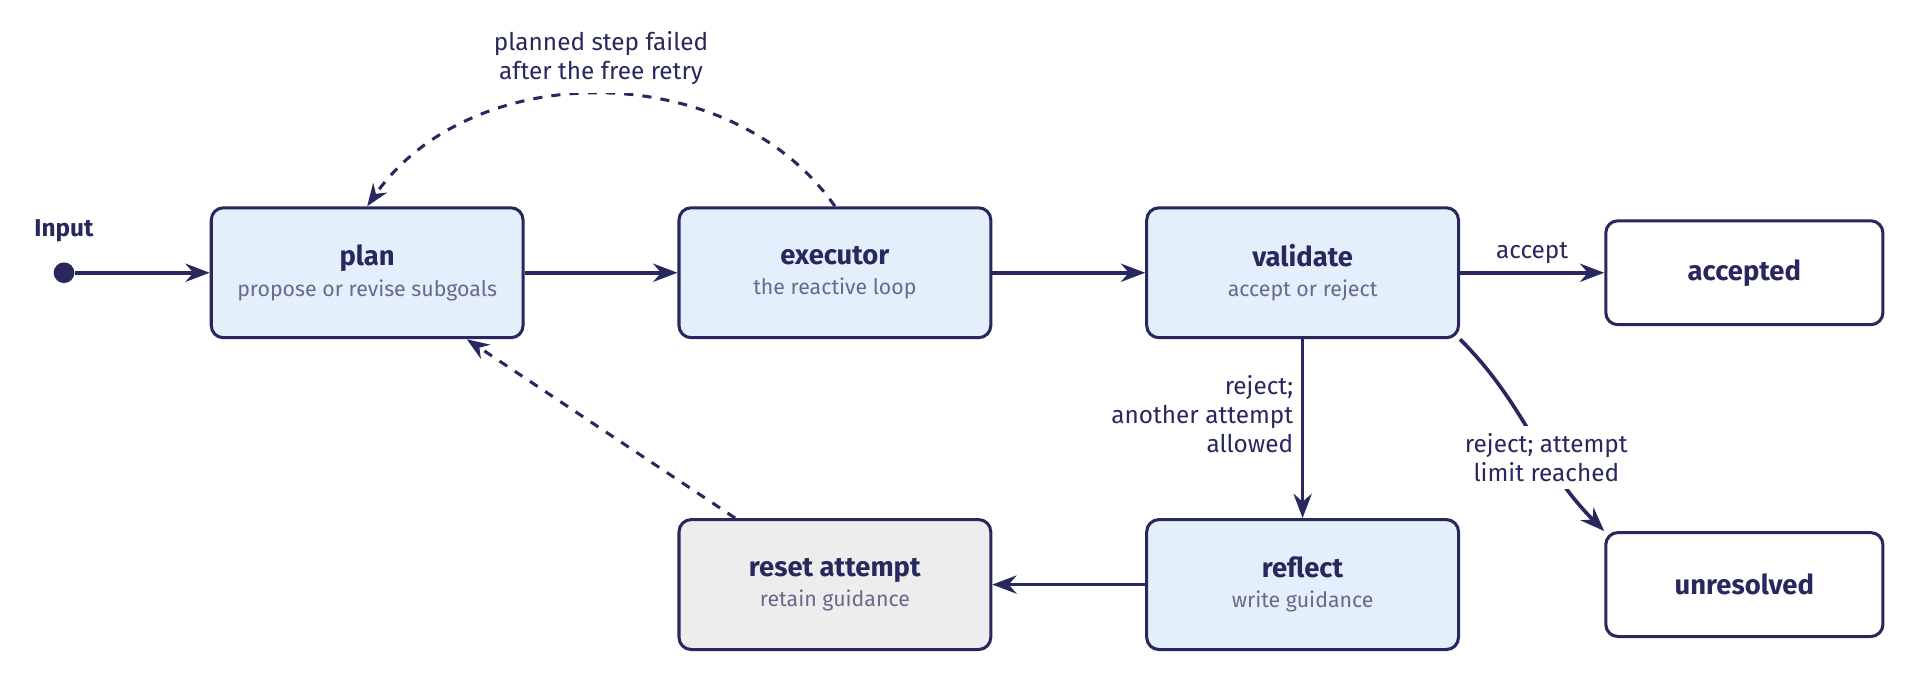
\includegraphics[width=\textwidth]{figures/deck/graph-complete.png}
  \caption{The complete graph of our agent, with the reactive loop drawn as the single node
  \texttt{executor}. The upper dashed edge, the in-run plan revision, is taken when the run stalls,
  by which time any failed tool call has had its free retry, and the lower dashed edge, through
  \texttt{reflect} and \texttt{reset attempt}, begins a new attempt.}
  \label{fig:control-graph}
\end{figure*}

\subsection{Where the next node is chosen}
\label{sec:control-routing}

Choosing the next node is split into three responsibilities, and each one belongs to a different
component. Recall that a node is one step of the graph, such as \texttt{controller},
\texttt{tools} or \texttt{plan}, which reads the state and returns an update (\cref{sec:state-record}).

\bi
\item \textbf{The model proposes.} The model produces values: a tool call, a plan, a candidate
patch, or a judgement about a patch. A proposal by itself does not change which node runs next.
\item \textbf{The runtime records.} The runtime merges each proposal into the state through the
reducers, the per-field merge functions of \cref{sec:state-transition}. It also writes what
happened to the trace (\cref{sec:state-records}).
\item \textbf{The router decides.} A routing function (\cref{sec:reactive-code}), which we call a
\textbf{router} for short, is a function we write that reads named fields of the state and returns
the name of the next node.
\ei

LangGraph, the framework in which our agent's graph is built, attaches a router to the graph as a
conditional edge.

\begin{definition}[Conditional edge]
\label{def:control-conditional-edge}
A conditional edge calls a routing function after a node runs: ``Similar to nodes, the
\texttt{routing\_function} accepts the current \texttt{state} of the graph and returns a value. By
default, the return value \texttt{routing\_function} is used as the name of the node (or list of
nodes) to send the state to next.''~\citep{langgraph-graph-api}
\end{definition}

A conditional edge therefore passes the current state to a routing function and sends the run to
the node whose name the function returns. The router is ordinary code that runs in the runtime's
process after the node finishes. The model never executes it. The run then enters the node that the
router names, which must be one of the successors we declared for that edge
(\cref{sec:reactive-code}).

The model still shapes the route, but only indirectly. Its output becomes part of the state, and
the router's comparisons read the state, so the model's output can decide which way a comparison
comes out. The comparison itself, and the set of nodes it may return, were written by us before the
run.

This division holds only while the router tests values with a fixed meaning, such as the
\demoref{status} field or whether the reply contains a tool call. Suppose instead that a router
searched the text of the model's reply for a phrase such as ``task complete''. The model could then
move the run by choosing its words. The control decision would in effect be the model's, even
though the code that returns the node name is still ours.

\subsection{The complete graph, with both back edges}
\label{sec:control-graph}

The complete graph of our agent places the planner, the validator and the reflection step around
the reactive loop (\cref{fig:control-graph}). The loop of \cref{sec:reactive}, with its
\texttt{controller}, \texttt{tools} and \texttt{submit} nodes, appears in the figure as the single
node \texttt{executor}. A run proceeds through the graph as follows.

\bi
\item \textbf{Plan.} The run enters at \texttt{plan}, which proposes subgoals at the start and
revises them when a planned step fails.
\item \textbf{Execute.} The \texttt{executor} runs the reactive loop, in which the model chooses
tool calls until it produces a candidate patch.
\item \textbf{Validate.} The \texttt{validate} node accepts or rejects the candidate. An accepted
candidate ends the run with the status \demoref{accepted}.
\item \textbf{Reflect and reset.} After a rejection, a router compares the number of attempts made
with the \textbf{attempt limit}, the largest number of attempts a run may make (two in our agent,
\cref{sec:control-limits}). If the run has made fewer attempts than the limit, it passes through
\texttt{reflect}, which writes guidance for the next attempt. It then passes through
\texttt{reset attempt}, which clears the attempt's working fields and keeps that guidance, and
returns to
\texttt{plan}. Once the attempt limit is reached, a rejection ends the run with the status
\demoref{unresolved}.
\ei

A back edge leads from a node to an earlier node of the graph, so that a run can return to a node
it has already visited (\cref{sec:reactive-graph}). The complete graph has two back edges into
\texttt{plan}:

\bi
\item \textbf{In-run plan revision.} The upper back edge, from \texttt{executor} to \texttt{plan},
revises the plan within an attempt. It is taken when the runtime has marked a planned step as
failed by setting the field \demoref{failed\_step}, which it does only when the run stalls for the
first time, that is, when three consecutive tool calls return the same observation
(\cref{sec:planning-stall}). Separately, when a single tool call fails, the runtime reissues it once
without calling the model. We call this the \textbf{free retry} (\cref{sec:control-owners}). A
failed tool call therefore never sends the run to the planner by itself. In code, the edge is one destination of the routing function after
the \texttt{tools} node, inside \texttt{executor}.
\item \textbf{New attempt after reflection.} The lower back edge, from \texttt{reset attempt} to
\texttt{plan}, begins a new attempt. It is reached through the reflection step and the reset, and
it returns the run to \texttt{plan} with the guidance from the failed attempt.
\ei

Every arrow in the figure is declared in the wiring code, the calls that add edges when the graph
is built. Every label on an arrow, such as ``reject; another attempt allowed'', names a predicate,
the condition in the code that selects a branch (\cref{sec:fixed-decisions}). In this graph, each predicate
is a test on fields of the state.

\subsection{What the router reads}
\label{sec:control-reads}

The router after \texttt{controller} tests two fields of the state and nothing else. It is the
routing function \demoref{after\_controller} of \cref{lst:reactive-after-controller}, which chooses
among the three successors of that node (\cref{sec:reactive-edge}).

If \demoref{status} holds anything other than \demoref{RUNNING}, the run has been given a terminal
status, and the function returns \demoref{END}, the framework's marker for the end of the graph.
Only the runtime writes \demoref{status}, for example when a limit fires. Otherwise the function
returns \texttt{tools} if the model's last message contains a tool call, and \texttt{submit} if it
does not, because the loop treats a reply without a tool call as a submission.

The router never reads the text of the model's reply. A reply that says ``I am confident, submit it'' and carries no tool call goes
to \texttt{submit}, exactly as an empty reply with no tool call does. A reply that says the work is
finished but carries a tool call goes to \texttt{tools}. The branch depends only on whether a tool
call is present.

The routing function after \texttt{submit}, \demoref{after\_submit}, makes a single test. It
returns \demoref{END} when the submission was accepted and \texttt{controller} otherwise, so a
rejected patch goes back to the model as feedback.

\subsection{Reading who decided from the trace}
\label{sec:control-who}

% Set here, ahead of the subsection that uses it, so that it reaches the page on which that
% subsection begins.
\begin{table*}[t]
  \centering
  \caption{The two returns to the planner: what triggers each back edge, which parts of the state
  it keeps, and which it clears.}
  \label{tab:control-backedges}
  \begin{adjustbox}{width=\linewidth}\begin{tabularx}{\linewidth}{@{}L{0.16\linewidth}L{0.24\linewidth}L{0.31\linewidth}X@{}}
    \toprule
    \textbf{Back edge} & \textbf{Trigger} & \textbf{Retained} & \textbf{Reset} \\
    \midrule
    \textbf{In-run plan revision} & The run stalls for the first time: three consecutive tool calls
      return the same observation, and the runtime sets \demoref{failed\_step}
      & The attempt's observations, and the counters \demoref{model\_calls} and \demoref{usage}
      & The remaining subgoals, which the planner rewrites \\ \addlinespace
    \textbf{New attempt after reflection} & The validator rejects and the attempt limit permits
      another try & Identity fields, \demoref{reflections}, the counters \demoref{model\_calls} and
      \demoref{usage}, and \demoref{attempt}
      & \demoref{observations}, \demoref{plan}, \demoref{candidate\_patch}, \demoref{validation} \\
    \bottomrule
  \end{tabularx}\end{adjustbox}
\end{table*}

Each time a router selects an edge, the runtime writes a routing event to the trace
(\cref{sec:reactive-edge}). The event's \demoref{decision} field records which branch was taken.
Its \demoref{by} field records who supplied the value that the routing predicate tested:

\bi
\item \textbf{\demoref{by="model"}.} The model's output selected the branch, because its reply
contained a tool call or contained none. The edges from \texttt{controller} to \texttt{tools} and
to \texttt{submit} are recorded this way.
\item \textbf{\demoref{by="runtime"}.} A field that the runtime owns selected the branch, for
example a limit that fired or the result of the submit checks.
\ei

A routing event with \demoref{by="model"} does not mean that the model decided the edge by itself.
The model supplied the value that was tested. The predicate that turns a tested value into a node
was written by us at design time, whichever value \demoref{by} holds. The \demoref{by} field
records only where the tested value came from.

When we say that the model of the reactive loop chooses the next node (\cref{sec:reactive-edge}),
we mean exactly this. The model supplies the value that \demoref{after\_controller} tests, and
\demoref{after\_controller}, which we wrote, turns that value into a node.

The routing events, and their \demoref{by} field in particular, are the first place to look when a
run behaves unexpectedly. Read in order, they show at every branch which way the run went and
whether a model output or a runtime field sent it there. That tells us where to look next: at what
the model produced, or at the limit or check that fired.

\subsection{One compiled graph, many paths}
\label{sec:control-paths}

A run can take many different paths through a graph that never changes. The graph is compiled
once, before any alert is read, and the same compiled object runs every alert
(\cref{sec:reactive-code}). Two runs on the same alert therefore run the same graph. They differ in
the sequence of states they pass through, and so in the sequence of edges that the routers select.

The wiring of the reactive loop shows where the paths of two runs can differ
(\cref{lst:reactive-edges}). Its two unconditional edges, from \demoref{START} to
\texttt{controller} and the back edge from \texttt{tools} to \texttt{controller}, are taken every
time the run reaches their source node (\cref{sec:reactive-graph}). The paths of two runs can
therefore differ only at the conditional edges after \texttt{controller} and \texttt{submit}.

A path, the sequence of nodes that one run actually visits (\cref{sec:reactive-code}), can thus
differ in length and shape from run to run, although the compiled graph is the same. In the example
run of the reactive loop (\cref{sec:reactive-run}), which was accepted after four model calls, the run
entered \texttt{controller} four times. A run on a harder alert would enter it more often, through
the same graph.

Paths differ because states differ, and states differ because each step consumes something from
outside the program. A model reply is sampled, so the same state can lead to different replies. A
tool result depends on the files, which the run itself may have edited (\cref{sec:state-diverge}).

Paths that vary from run to run therefore do not require a graph that varies from run to run. The
same routers read a different state on each run, and so select different edges. The task
environment itself is still deterministic, since the same read on the same files returns the same
result (\cref{sec:agents-properties}).

\subsection{Two returns to the planner}
\label{sec:control-backedges}

The two back edges into \texttt{plan} (\cref{fig:control-graph}) answer different questions, and
they must remain separate. The in-run plan revision asks what to do about a step that did not work.
The new attempt after reflection asks what to do about an attempt that did not work, that is, a
whole pass of planning, execution and validation that ended in a rejected patch. Neither edge
exists in the reactive loop. Both are added to the graph together with the planner and the
reflection step.

The two edges differ in what triggers them, in which fields of the state they keep, and in which
fields they clear (\cref{tab:control-backedges}). Compare the Retained and Reset columns across the
two rows.

The in-run plan revision keeps everything the attempt has learned. The observations stay, and so do
the counters \demoref{model\_calls} and \demoref{usage}, which count the model calls and the tokens
spent. The planner rewrites only the subgoals that remain, using the evidence the attempt has
gathered.

The new attempt keeps much less. It retains the reflections, which hold the guidance written after
the rejection. It retains the identity fields, which are set once at the start: the alert, the
repository, the commit and the workspace. It also retains the counters \demoref{model\_calls} and
\demoref{usage}, and the attempt counter \demoref{attempt}, because they cover the whole run.

The new attempt clears the observations, the plan, the candidate patch and the validation result.
The next attempt therefore starts without the reasoning that failed, but with the guidance about
it. Clearing a field that has an append reducer, such as \demoref{observations}, takes an explicit
assignment by the runtime, because an update merged through that reducer can only add items
(\cref{sec:state-reset}).

The two edges must stay distinct because they respond to different kinds of failure: a step that
did not work, and an attempt that ended in a rejected patch. Each edge has its own trigger. The
in-run plan revision is reached only after a stall, which the runtime records in
\demoref{failed\_step}, and the new attempt only after the validator's rejection.

A tool error may be \textbf{transient}, that is, it may not recur if the same call is simply
repeated. A transient error is not evidence that the plan is wrong, so the runtime absorbs it with
the free retry, and neither back edge is taken. If the two returns were merged into one, a single
trigger would have to stand for every kind of failure. The system could then no longer tell a failed
step from a failed attempt, and any failure, including a transient tool error, would send the run
back to rewrite its plan. Rewriting the plan costs a model call and can replace a plan that was
sound.

\subsection{Who owns each return}
\label{sec:control-owners}

Ownership of the returns follows the division of responsibilities in \cref{sec:control-routing}:
the model proposes values, and the decisions belong to code we wrote, in the runtime and in our
routers. Three decisions are involved.

\bi
\item \textbf{Free retry.} The runtime owns the free retry. When a tool call fails, the runtime
reissues it once, because a transient failure is not evidence about the plan.
\item \textbf{In-run plan revision.} The model proposes the revision. Once the runtime has decided
that a planned step has failed, it records that decision in the field \demoref{failed\_step}, which
the model never writes (\cref{sec:planning-stall}). The run returns to \texttt{plan}, where the
model proposes new remaining subgoals, and the runtime merges the proposal into the \demoref{plan}
field.
\item \textbf{New attempt.} The decision to start a new attempt belongs to a router we wrote. It
compares the attempt counter, the field \demoref{attempt}, with the attempt limit.
\ei

The retry is called free because it costs no model call. The runtime repeats the tool call without
consulting the model, so the retry adds nothing to the count of model calls or to the tokens used.
Because no model output is involved, the retry is the runtime's decision rather than the model's.

The new attempt belongs to code we wrote for a different reason. If the model's output decided
whether another attempt runs, the model could argue for one more attempt every time, and the number
of attempts would have no upper bound. A limit enforced by comparing a counter that the model
cannot write is one that no model output can change.

\subsection{Limits that the runtime checks}
\label{sec:control-limits}

The \textbf{acceptance condition} of our agent is the set of checks that a patch must pass to be
accepted. It says when a run may stop, but it does not ensure that the run will stop, because a run
that never produces an acceptable patch never satisfies it. Three limits, checked by the runtime,
are designed to make every run stop. Each limit is a comparison that the runtime performs on a
field it owns:

\bi
\item \textbf{The budget.} A run may make at most forty model calls. The
\texttt{controller} node checks the count of model calls, \demoref{model\_calls}, before it issues
each call. A check made after the call would come too late, because the call would already have
been made and paid for. A run stopped by the budget therefore records no further model call after
its last routing event.
\item \textbf{The stall check.} In the reactive loop, the run ends after three consecutive
observations with identical results. With the planner, the first such stall triggers the in-run
plan revision, and a second one ends the run (\cref{sec:planning-stall}).
\item \textbf{The attempt limit.} A run may make at most two attempts. The attempt counter is kept
in a field that survives the reset between attempts (\cref{tab:control-backedges}). A counter that
was reset with the attempt would return to its starting value at every attempt, so the limit would
never be reached.
\ei

The stall check compares results rather than requests (\cref{sec:reactive-stops}). It therefore
catches a model that repeats the same request on files that have not changed, because the same read
on the same files returns the same result (\cref{sec:agents-properties}). It also catches a model
that varies its requests without effect, for example by searching with several different patterns
that each return no matches. A model that repeats its earlier actions is a known failure: the
published ReAct agent, in some of its runs, repeated its earlier thoughts and actions without making
progress \citep{yao2023react}. On unchanged files, such repetition returns identical results, which
the stall check catches.

The stall check catches only one form of non-progressive iteration (\cref{sec:reactive-shapes}),
the form in which the results repeat exactly. Other forms go undetected while the run is in
progress.

In the reactive loop, the budget and the stall check sit in the code of the \texttt{controller}
node, before the model call (\cref{sec:reactive-stops}). The attempt limit is tested by the routing
function after \texttt{validate}.

In addition to these three limits, the framework enforces its own \textbf{recursion limit}:
LangGraph caps the number of super-steps a single run may execute. A \textbf{super-step} is one
round of node executions, and in our graph, whose nodes run one at a time, it is one node
execution. When the cap is reached, LangGraph raises a \demoref{GraphRecursionError} instead of
routing to \demoref{END}, so the run stops with an exception that our code must catch to record a
terminal status. The cap guards against a mistake in the wiring, such as a cycle in the graph that
none of our limits covers. It does so only if it is set above the number of steps that a correctly
wired run can take within forty model calls. Our three limits then end every correctly wired run,
and the recursion limit fires only if the wiring is wrong.

\subsection{Terminal statuses}
\label{sec:control-statuses}

Recall that a run's terminal status is the value of the \demoref{status} field that records how it
ended (\cref{sec:state-schema}). Our agent uses a closed set of five terminal statuses: every
terminal status that the runtime records is one of them, and no other value is allowed. Because the
set is closed, a reader of a trace knows every possible outcome in advance, and the outcomes of
different runs can be counted and compared.

\bi
\item \textbf{Introduced with the reactive loop.} The status is \demoref{accepted} when the patch
satisfied the acceptance condition, \demoref{budget\_exhausted} when the budget ran out,
\demoref{no\_progress} when the stall check fired, and \demoref{error} when the run stopped on a
failure it could not recover from.
\item \textbf{Introduced with the attempt limit.} The status is \demoref{unresolved} when the
validator rejected the patch of the last allowed attempt.
\ei

We call the four statuses other than \demoref{accepted} \textbf{stop statuses}. Each records that
the run ended without an accepted patch.

A \textbf{terminal event} is the event that records the run's terminal status, and it is the last
event of a complete trace. The \textbf{trace writer}, the component that writes events to the
trace, refuses two mistakes. It rejects a status outside the set, and it rejects a trace that is
closed without a terminal event.

Because of these checks, our runtime cannot close a trace normally without recording how the run
ended. If our code ever ended a run without recording its ending, that would be a defect in the
code that writes the trace. It would not be an outcome we could report. A trace can still lack a
terminal event when the process stops before the trace is closed, for example when the process is
killed (\cref{sec:control-conclude}).

Errors inside a run and the outcome of a run are different things. A refused tool call is an error
inside the run: it becomes an observation that the model reads (\cref{sec:boundary}), and the run
can still end \demoref{accepted}. The terminal status \demoref{error} is reserved for a failure that
ends the run. A process that is killed between two events is a third case, because it leaves the
run with no terminal status at all.

Reaching \demoref{END} shows only that the graph stopped. It does not say why. The reason is in the
\demoref{status} field, which our runtime sets.

\subsection{What a trace lets us conclude}
\label{sec:control-conclude}

What we may conclude about a run depends on what its trace records at the end. A
\textbf{verdict} is the recorded decision to accept or reject a patch. \Cref{tab:control-conclude}
pairs each way a trace can end with the conclusion it supports. Read each row as a limit on what may
be claimed.

\begin{table}[htbp]
  \centering
  \caption{What a trace lets us conclude, by what the trace records at its end.}
  \label{tab:control-conclude}
  \begin{adjustbox}{width=\linewidth}\begin{tabularx}{\linewidth}{@{}L{0.36\linewidth}X@{}}
    \toprule
    \textbf{What the trace records} & \textbf{What it supports} \\
    \midrule
    \textbf{A verdict, then a terminal event with status \demoref{accepted}} & A run completed under
      our acceptance condition. Whether the patch is a good fix is a separate question \\
      \addlinespace
    \textbf{A terminal event with a stop status and its reason} & A declared end to execution, with
      whatever partial evidence the run had gathered \\ \addlinespace
    \textbf{No terminal event} & Completion has not been established by this record \\
    \bottomrule
  \end{tabularx}\end{adjustbox}
\end{table}

\bi
\item \textbf{A verdict and \demoref{accepted}.} This trace shows that the run completed under our
acceptance condition. Whether the patch is a good fix is a separate question, because the checks
test less than the performance measure asks (\cref{sec:fixed-costs}).
\item \textbf{A stop status.} A terminal event with \demoref{budget\_exhausted},
\demoref{no\_progress}, \demoref{error} or \demoref{unresolved} shows a declared end to
execution: the runtime stopped the run and recorded the reason. The evidence the run gathered up to
that point remains in the record, though it is partial.
\item \textbf{No terminal event.} This trace does not establish that the run completed. The run may
still be active, it may have been interrupted, or it may have written an incomplete trace, and the
record does not say which.
\ei

A missing terminal event therefore tells us only that the record is incomplete. Reporting the run as
failed, or as ending with the status \demoref{error}, would attribute a cause that the record does
not contain.

\subsection{Three endings}
\label{sec:control-endings}

Three example endings show how the rows of \cref{tab:control-conclude} apply. Each one leaves a
different event as the last event of its trace.

\bi
\item \textbf{Accepted.} The last event is a terminal event with the status \demoref{accepted} and
the run's usage totals. In the reactive loop, it is written after the \texttt{submit} node reports
that all three checks passed: the patch applies, it touches the flagged line, and the rescan is
clean. In the complete graph, the \texttt{validate} node makes this decision instead
(\cref{sec:control-graph}).
\item \textbf{Budget exhausted.} The budget check fires before the model call, so no further model
call is recorded between the last routing event and the terminal event. The evidence the run
gathered remains in \demoref{observations}. A run that ends without an accepted patch may still
have done substantial work, and its observations show what it examined.
\item \textbf{No ending observed.} The run is interrupted between a tool result and the next model
call. Every event in the trace is valid, and no terminal event arrives.
\ei

In the accepted example run of the reactive loop (\cref{sec:reactive-run}), the routing event just
before the terminal event carries \demoref{by="runtime"}, because the value tested was the result
of the checks. The run therefore ended on the result of the checks, and no statement by the model
about whether the work was done entered that decision.

For the interrupted run, we cannot say which ending would have arrived. The trace also does not
record that the run was interrupted. From the record alone, it is a trace with no terminal event
(\cref{tab:control-conclude}). For this reason, a trace excerpt shown as an example should be
labeled with how it was produced, for example as a complete run or as an interrupted one.

\subsection*{Key points}
\bi
\item The model proposes values and the runtime records them, while a router we wrote decides the
next node by testing named fields of the state, because a router that read the text of the model's
reply would give the control decision to the model.
\item A routing event's \demoref{by} field records whether the model's output or a field the runtime
owns supplied the tested value, and in either case the predicate was written by us.
\item The graph is compiled once and is the same object on every run, and runs take different paths
because their states differ, so the routers select different edges.
\item The in-run plan revision responds to a failed step and keeps the attempt's observations, while
the new attempt after reflection responds to a rejected patch and clears the attempt's working
fields.
\item The runtime owns the free retry, a router we wrote owns the decision to start a new attempt,
and the model only proposes the revised subgoals.
\item The runtime is designed to stop every run with three limits on fields it owns: a budget of
forty model calls checked before each call, a stall check on three identical results, and an
attempt limit of two counted in a field that survives the reset.
\item Reaching \demoref{END} shows only that the graph stopped, so the reason is recorded as one of
five terminal statuses, and a trace without a terminal event does not establish whether the run
completed.
\ei
